%%%%%%%%%%%%%%%%%%%%%%%%%%%%%%%%%%%%%%%%%%%%%%%%%%%%%%%%%%%%%%%%%%%%%%%%%%%%%%%%
% Evidence-aligned draft, 2026-10-15.
% Implementation: 58373240451d6ab093c7e3a154164a94f9dabab3.
% Reported results: resetfix and phasebalanced climb, seed 0, 3000 iterations.
% This draft does not import the older manuscript's six-motion/five-seed table.
%%%%%%%%%%%%%%%%%%%%%%%%%%%%%%%%%%%%%%%%%%%%%%%%%%%%%%%%%%%%%%%%%%%%%%%%%%%%%%%%
\documentclass[letterpaper,10pt,conference]{ieeeconf}
\IEEEoverridecommandlockouts
\overrideIEEEmargins
\usepackage{amsmath,amssymb,booktabs,graphicx,cite,url,newtxtext,newtxmath,microtype,flushend}
\emergencystretch=1em
\XeTeXtracingfonts=0
\title{\LARGE\bf DARE: Differential Adversarial Reward Equalization for Humanoid Motion Imitation}
\author{Anonymous Authors}

\begin{document}
\maketitle
\thispagestyle{empty}
\pagestyle{empty}

\begin{abstract}
Physics-based humanoid motion imitation requires tracking root position,
joint rotation, body position, and other motion quantities. Handcrafted
rewards combine these errors using manually selected weights and scales,
which can require adjustment when the reference motion changes. We propose
DARE, Differential Adversarial Reward Equalization, to learn a tracking
reward without motion-specific reward coefficients. DARE processes the
complete reference--policy difference, normalizes its coordinates using
observed errors, and uses a convex-potential discriminator to control
sensitivity without a gradient-penalty coefficient. During policy learning,
phase weights are computed from observed sample counts rather than manually
assigned to particular motion stages. A controlled climb experiment shows
earlier full-motion completion and lower final tracking errors under the
same training budget. The approach brings reward learning and automatic
phase balancing into one training procedure designed for reuse across
reference motions.
\end{abstract}

\section{Introduction}
Physics-based motion imitation learns a controller that reproduces a
reference motion while respecting dynamics, actuator limits, and contact.
The controller must track several quantities at once, including root
position, joint rotation, and body position. A common approach converts
each tracking error into a separate reward term and combines the terms
with chosen weights. These choices determine how strongly different
errors affect policy learning. Finding suitable coefficients can become
an additional engineering task whenever a new motion is introduced.

Our aim is to reduce this motion-specific work: changing the reference
motion should not require redesigning its tracking reward or assigning
special priorities to selected motion stages. This is a shared-configuration
goal. Network sizes, optimizer settings, and the training budget are fixed
in advance; tracking coefficients are not selected separately for each
motion.

Adversarial imitation provides a learned alternative to handcrafted reward
aggregation. AMP learns a motion prior from reference transitions
\cite{peng2021amp}. ADD uses the synchronized reference--policy differential
to learn a tracking reward, with perfect tracking represented by a zero
differential \cite{zhang2025add}. This removes explicit component-wise
tracking weights. However, controlling the discriminator through a
gradient penalty introduces a coefficient that trades off classification
and input sensitivity. ADD's humanoid experiments use a different
gradient-penalty coefficient for Climb than for the other motions
\cite{zhang2025add}. Structural sensitivity constraints offer a way to
remove this reward-learning coefficient from motion-specific selection.

DARE builds on differential adversarial learning and uses a
convex-potential discriminator. Its normalized input retains the complete
tracking difference. Convex-potential layers constrain how strongly
input changes can affect the hidden representation, while their residual
form supports a deep discriminator \cite{meunier2022cpl}. The discriminator
learns one score from the joint errors, rather than fitting a prescribed
scalar formula for motion quality.

Reward learning alone does not determine how different stages contribute
to policy training. Random reference-state initialization improves motion
coverage \cite{peng2018deepmimic}, but the collected transitions can still
have unequal phase frequencies because episodes advance and terminate.
DARE therefore computes phase weights from each rollout's sample counts.
The same rule is used for advantage normalization and the Actor and Critic
losses. No motion-specific list of difficult stages or stage priorities is
provided.

The method combines two mechanisms around one goal: learning the tracking
reward without manually chosen tracking coefficients, and improving the
use of that reward without manually chosen stage weights. We present the
implementation and a controlled climb study that measures learning speed,
full-motion execution, and seven physical tracking errors. The evaluation
is organized around learning efficiency and accuracy under a fixed
configuration.

The design contributions are a deep, structurally constrained differential
discriminator that removes gradient-penalty selection, and rollout-driven
phase balancing that computes update weights with one motion-independent
rule. Their shared purpose is reliable reference tracking without
motion-specific reward engineering.

\section{Related Work}
\textbf{Physics-based motion imitation.}
DeepMimic learns reference-guided skills using explicit tracking rewards
and random reference-state initialization \cite{peng2018deepmimic}.
Such rewards make the desired tracking quantities clear, but their weights
and error scales must be specified. Our focus is replacing those
coefficients with a learned reward while retaining reference-conditioned
control.

\textbf{Learned imitation rewards.}
GAIL learns an imitation objective by distinguishing expert and policy
behavior \cite{ho2016gail}. AMP learns rewards from reference motion
transitions \cite{peng2021amp}. ADD directly classifies the synchronized
reference--policy difference against the ideal zero differential
\cite{zhang2025add}. DARE builds on this differential formulation with a
constrained discriminator and automatically weighted policy training.

\textbf{Constrained discriminators.}
Gradient penalties and spectral normalization control discriminator
sensitivity \cite{gulrajani2017improved,miyato2018spectral}. Convex-potential
layers provide non-expansive residual transformations
\cite{meunier2022cpl}. We adapt this existing construction to the deep
differential discriminator, replacing a separately weighted gradient
penalty with a structural constraint.

\section{Background}
Let $s_t$ and $\hat s_t$ denote the policy state and synchronized reference
state at time $t$. A feature extractor $\phi$ collects the tracked
quantities. A representative handcrafted reward partitions them into $G$
groups and combines their errors as
\begin{equation}
r_t^{\mathrm{hand}}=\sum_{g=1}^{G}w_g
\exp\!\Bigl[-\alpha_g
\bigl\|\phi_g(\hat s_t)-\phi_g(s_t)\bigr\|_2^2\Bigr].
\label{eq:hand}
\end{equation}
Here, $w_g$ determines a group's contribution and $\alpha_g$ determines
how rapidly its reward decreases with error. DARE replaces this
component-wise reward construction with a learned discriminator score.
The policy and value function are trained using PPO and TD-$\lambda$
returns \cite{schulman2017ppo,schulman2016gae}.

\begin{figure*}[t]
\centering
\setlength{\tabcolsep}{5pt}
\begin{tabular}{@{}c c c c c c c@{}}
\fbox{\parbox[c][0.52in][c]{0.17\textwidth}{\centering
Synchronized reference\\and policy states}}
& $\longrightarrow$ &
\fbox{\parbox[c][0.52in][c]{0.17\textwidth}{\centering
Normalized tracking\\differential $\Delta_t$}}
& $\longrightarrow$ &
\fbox{\parbox[c][0.52in][c]{0.17\textwidth}{\centering
Convex-potential\\discriminator reward}}
& $\longrightarrow$ &
\fbox{\parbox[c][0.52in][c]{0.17\textwidth}{\centering
Automatically phase-\\weighted PPO}}
\end{tabular}
\caption{DARE's reward and policy-update path. A synthetic zero differential
and current/replay policy differentials train the discriminator. Phase
weights are calculated from rollout counts and affect policy/value updates,
not discriminator labels.}
\label{fig:pipeline}
\end{figure*}

\section{DARE}
\subsection{Learned Differential Reward}
DARE constructs the normalized differential at time $t$ as
$\Delta_t=\mathcal N\!\left(\phi(\hat s_t)-\phi(s_t)\right)$.
Rotations use a tangent--normal representation so that their differences
are expressed in Euclidean coordinates.

The tracked quantities use different units and numerical scales,
with position errors measured in meters, linear-velocity errors in meters
per second, and angular-velocity errors in radians per second. Directly
feeding these values to the discriminator can make numerically larger
coordinates dominate its input. Following the differential normalization
used in ADD, the normalizer divides each coordinate by its accumulated
mean absolute residual. The resulting values are dimensionless and have
comparable numerical magnitudes before discriminator processing. Statistics
are estimated during early training and fixed after $10^8$ samples.

Perfect tracking gives the positive sample $\Delta^+=0$. Policy
differentials form the negative samples $\Delta^-$. Stored reference--policy
pairs are also sampled from a replay buffer, allowing their differences
to be normalized consistently with the current rollout. The scalar
discriminator $f_\theta$ maps a normalized differential to a logit,
meaning its real-valued score before the sigmoid function. It is trained
using the balanced binary logistic loss
\begin{align}
\mathcal L_D(\theta)
&=\tfrac12\operatorname{softplus}\!\left[-f_\theta(0)\right]
\notag\\
&\quad+\tfrac12\operatorname{mean}_{\Delta^-}
\operatorname{softplus}\!\left[f_\theta(\Delta^-)\right].
\label{eq:disc}
\end{align}
The mean is taken over equal numbers of current and replay negative
samples. The first term increases the zero differential's score; the
second decreases the policy differentials' scores. All tracking
coordinates are processed jointly, allowing the score to depend on their
individual values and interactions.

The implemented policy reward is
\begin{equation}
r_t^{\mathrm{DARE}}=-2\log\max\!\left\{
1-\sigma\!\left(f_\theta(\Delta_t)\right),10^{-4}\right\}.
\label{eq:reward}
\end{equation}
Until the cap is reached, this equals
$2\operatorname{softplus}(f_\theta(\Delta_t))$: a higher score gives a
higher reward. The multiplier is fixed for the shared configuration. No
separate root, pose, or velocity tracking reward is added.

\subsection{Convex-Potential Discriminator}
The discriminator uses a structural sensitivity constraint instead of a
gradient penalty. Spectral normalization controls linear-map gain, and
the hidden trunk uses the convex-potential construction of Meunier
et al.\ \cite{meunier2022cpl}. Each block maps a hidden vector $h$ to
\begin{equation}
C_\ell(h)=h-2\bar W_\ell^{\mathsf T}
\operatorname{ReLU}(\bar W_\ell h+b_\ell),
\qquad \|\bar W_\ell\|_2\leq1.
\label{eq:cpl}
\end{equation}
The transpose is tied to the same weight matrix. Under the stated
spectral-norm bound, this transformation is non-expansive: changing the
input by a given Euclidean distance cannot change the output by a larger
distance. Its identity path also carries hidden information through the
trunk, rather than relying solely on repeated affine--ReLU transformations.

The frontend encodes seven disjoint tracking groups: root position, root
rotation, body-relative position, body rotation, root linear velocity,
root angular velocity, and joint velocity. Each group receives the same
embedding width, and the embeddings are concatenated before fusion.
These are feature encoders, not separately weighted reward terms.
All frontend, fusion, and scalar-output linear maps use spectral
normalization. Because the input groups are disjoint, concatenating
non-expansive group encodings is also non-expansive in the joint Euclidean
norm. Composing these encoders, fusion, CPL blocks, and output gives the
ideal bound $|f_\theta(\Delta)-f_\theta(\Delta')|
\leq\|\Delta-\Delta'\|_2$.

This construction limits score sensitivity without selecting a
gradient-penalty coefficient. In the implementation, spectral norms are
estimated by one power iteration per training forward; the ideal bound
describes the exact-normalization construction, not a numerical
certificate for every trained weight matrix.

\subsection{Automatic Phase Balancing}
Random-phase initialization exposes the policy to different parts of the
reference motion. However, the frequency of collected transitions also
depends on episode duration, advancement, and early failure. Uniformly
averaging those transitions gives frequently visited phases more influence
on the update.

DARE divides normalized motion phase into eight equal intervals, with the
same division rule for every motion. Let $n_b$ be the number of rollout
transitions in interval $b$, $N$ the total number of transitions, and
$B_+$ the number of intervals containing samples. A transition from an
occupied interval receives weight
\begin{equation}
w_b=\frac{N}{B_+n_b}.
\label{eq:phase}
\end{equation}
Summing these weights within an interval gives $N/B_+$, so every observed
interval contributes the same total weight. Rarely sampled intervals
receive larger per-transition weights, without a manually specified
priority for any particular stage.

For a per-transition loss, the resulting full-rollout weighted average
equals the arithmetic mean of the occupied intervals' individual average
losses. This gives each observed part of the reference equal contribution
by construction, instead of letting its contribution be set by how often
the current policy happens to visit it. The eight-interval partition is
fixed globally; only the measured counts and resulting weights change.

The weights are used to compute the mean and standard deviation for
advantage normalization. Actor training minimizes the weighted PPO
clipped loss, while Critic training minimizes weighted squared error to
TD-$\lambda$ targets. Minibatches still sample transitions uniformly;
the weights change their contributions after sampling. The discriminator
retains the binary objective in Eq.~\eqref{eq:disc}. This mechanism
balances the use of already collected data; it does not replace missing
experience or provide motion-quality labels.

\subsection{Training Procedure}
Each iteration collects a synchronized rollout using random reference-state
initialization and sampled policy actions. Selected reference--policy pairs
are inserted into replay. The current discriminator supplies rewards before
the model updates. TD-$\lambda$ targets, advantages, and phase weights
are then computed. The implementation updates the Critic and Actor, followed
by the discriminator using current and replay negatives. Early-training
normalization statistics are updated after these model updates.
Evaluation restores training mode before subsequent training resets.
The discriminator, reward definition, and phase-weight rule are shared;
the reference motion supplies the task-specific trajectory.

\section{Verified Climb Study}
\subsection{Setup and Evidence Scope}
The climb comparison uses the same robot and reference motion, with 8192
environments, 32-step rollouts, and a 3000-iteration budget using seed 0.
The baseline is the reset-corrected CPL-DARE run without phase balancing.
The compared version adds weighted advantage normalization and weighted
Actor/Critic losses. Reward construction, discriminator, normalization
budget, action noise, and random-phase initialization are unchanged.
Thus this study isolates the phase-balancing package, not its three
internal uses individually.

Actor and Critic MLPs have hidden widths 1024 and 512. The discriminator
has seven 146-channel group encoders, a 1022-to-512 fusion layer, seven
512-channel CPL blocks, and one scalar output. PPO uses clip 0.2,
discount 0.99, TD-$\lambda$ 0.95, and fixed action standard deviation
0.05. Actor, Critic, and discriminator use 5, 2, and 2 training epochs
per rollout. SGD learning rates are $10^{-4}$ for Actor and Critic and
$2.5\times10^{-4}$ for the discriminator. Replay capacity is 200000 pairs.

Fixed-start evaluation executes mean actions from the first reference
frame. A length of 299 steps corresponds to completing this motion under
the original termination rules. Completion and tracking accuracy are
reported separately. The seven errors are the final logged evaluation
metrics, with body position measured relative to the root. Results below
are single-seed observations, not means or confidence intervals across
independent training runs.

\subsection{Learning Efficiency and Tracking}
Figure~\ref{fig:climb_learning} compares the recorded evaluations at the
same sample budgets. It shows full-motion execution separately from root
position and joint-velocity tracking, so that completing the reference
does not conceal remaining physical errors.

\begin{figure*}[t]
\centering
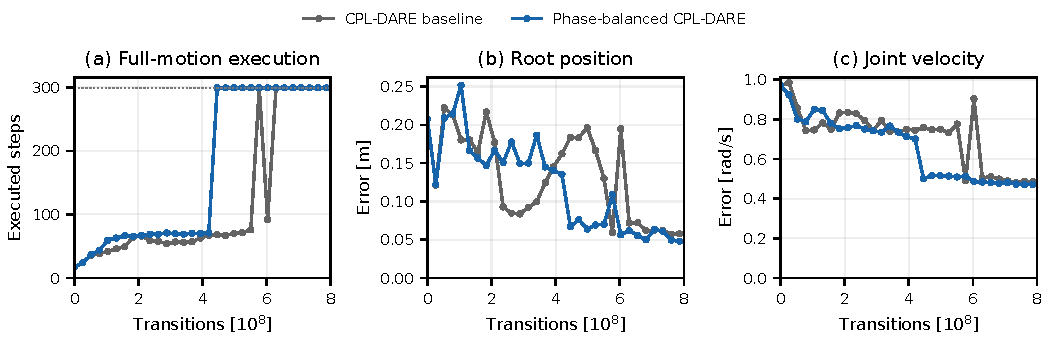
\includegraphics[width=0.94\textwidth]{figures/dare_fixed_config_climb.pdf}
\caption{Climb learning curves from the two seed-0 runs used in
Table~\ref{tab:climb}. Dots are recorded evaluations, separated by 100
iterations except for the final checkpoint; lines only connect those
records. Errors are averaged over each policy's executed evaluation
trajectory, which can have different lengths during learning. The dotted
line in panel (a) marks the 299-step full-motion length.}
\label{fig:climb_learning}
\end{figure*}

The first logged full-motion evaluation occurs at iteration 2200 for
the baseline and 1700 with phase balancing. These correspond to
576978944 and 445906944 collected transitions, respectively, a difference
of 131072000 transitions. Evaluations are separated by 100 iterations,
so these are first observed completion points rather than exact learning
times. All 14 recorded evaluations from iteration 1700 to 2999 in the
phase-balanced run execute 299 steps; the baseline falls to 92.16 steps
at iteration 2300 before recovering.

\begin{table}[t]
\caption{Final logged climb errors, seed 0, under the same 3000-iteration
budget. Reduction is relative to the baseline.}
\label{tab:climb}
\centering
\footnotesize
\setlength{\tabcolsep}{3pt}
\begin{tabular}{lrrr}
\toprule
Metric & Baseline & Balanced & Reduction \\
\midrule
Root position [m] & 0.05791 & 0.04814 & 16.87\% \\
Root rotation [rad] & 0.03901 & 0.03568 & 8.52\% \\
Body position [m] & 0.02257 & 0.01999 & 11.46\% \\
Body rotation [rad] & 0.08349 & 0.07565 & 9.40\% \\
Joint velocity [rad/s] & 0.48545 & 0.47226 & 2.72\% \\
Root velocity [m/s] & 0.11252 & 0.10223 & 9.14\% \\
Root ang. velocity [rad/s] & 0.26740 & 0.25220 & 5.68\% \\
\bottomrule
\end{tabular}
\end{table}

All seven final errors decrease in this run, as shown in
Table~\ref{tab:climb}. Completion does not eliminate intermediate accuracy
variation: root-position error is 0.1089 m at iteration 2200 in the
phase-balanced run, despite full-motion execution, and falls to 0.0481 m
at the final checkpoint. The learning curve also retains a long platform
near 70 steps before iteration 1700. These observations motivate measuring
both sample efficiency and physical accuracy, rather than using episode
length as the sole outcome.

\subsection{Evaluation Required for the Shared-Configuration Claim}
The main research question is whether the same method works across motions
without selecting new reward coefficients. That question requires
from-scratch training on motions with different durations and contacts,
using the configuration frozen before observing their results. Independent
seeds must be the statistical unit. A common protocol should report
completion, seven tracking errors, and transitions to a predeclared
completion criterion, while recording any changes to configurations.
Necessary scene assets and the reference motion should be distinguished
from reward or training-parameter changes.

Component comparisons should retain the same reward, budget, and evaluation
conditions. A discriminator comparison tests the benefit of CPL against
gradient-penalty and plain spectrally normalized alternatives; a policy
comparison isolates phase balancing. Separate advantage, Actor, and Critic
ablations can determine which parts of balancing drive the observed effect.
The verified climb result supports this evaluation program but does not
establish cross-motion reliability or three separate causal effects.

\section{Conclusion}
DARE combines differential reward learning, a convex-potential discriminator,
and automatically computed phase weights around a shared-configuration
motion-imitation objective. It replaces manually weighted tracking rewards
with one learned score and removes the discriminator's gradient-penalty
coefficient. Phase contributions are calculated from rollout frequencies,
rather than assigned separately for each motion. The verified climb study
shows earlier observed completion and lower final tracking errors for
the phase-balanced version. Demonstrating that this configuration reliably
transfers to different reference motions remains the central requirement
for the broader no-motion-specific-tuning claim.

\begin{thebibliography}{99}
\bibitem{peng2018deepmimic}
X.~B. Peng, P.~Abbeel, S.~Levine, and M.~van~de~Panne, ``DeepMimic:
Example-guided deep reinforcement learning of physics-based character
skills,'' \emph{ACM Trans. Graph.}, vol.~37, no.~4, 2018.
\bibitem{ho2016gail}
J.~Ho and S.~Ermon, ``Generative adversarial imitation learning,'' in
\emph{Advances in Neural Information Processing Systems}, 2016.
\bibitem{peng2021amp}
X.~B. Peng, Z.~Ma, P.~Abbeel, S.~Levine, and A.~Kanazawa, ``AMP: Adversarial
motion priors for stylized physics-based character control,''
\emph{ACM Trans. Graph.}, vol.~40, no.~4, 2021.
\bibitem{zhang2025add}
Z.~Zhang, S.~Bashkirov, D.~Yang, Y.~Shi, M.~Taylor, and X.~B. Peng,
``Physics-based motion imitation with adversarial differential
discriminators,'' in \emph{SIGGRAPH Asia Conf. Papers}, 2025.
\bibitem{gulrajani2017improved}
I.~Gulrajani, F.~Ahmed, M.~Arjovsky, V.~Dumoulin, and A.~Courville,
``Improved training of Wasserstein GANs,'' in \emph{Advances in Neural
Information Processing Systems}, 2017.
\bibitem{miyato2018spectral}
T.~Miyato, T.~Kataoka, M.~Koyama, and Y.~Yoshida, ``Spectral normalization
for generative adversarial networks,'' in \emph{Proc. ICLR}, 2018.
\bibitem{meunier2022cpl}
L.~Meunier, B.~J. Delattre, A.~Araujo, and A.~Allauzen, ``A dynamical system
perspective for Lipschitz neural networks,'' in \emph{Proc. ICML},
pp.~15484--15500, 2022.
\bibitem{schulman2017ppo}
J.~Schulman, F.~Wolski, P.~Dhariwal, A.~Radford, and O.~Klimov,
``Proximal policy optimization algorithms,'' arXiv:1707.06347, 2017.
\bibitem{schulman2016gae}
J.~Schulman, P.~Moritz, S.~Levine, M.~Jordan, and P.~Abbeel,
``High-dimensional continuous control using generalized advantage
estimation,'' in \emph{Proc. ICLR}, 2016.
\end{thebibliography}
\end{document}
